%=========================================================================
% sec-opts-avx
%=========================================================================

\section{Vectorizing with SIMD Extensions}
\label{sec-opts-avx}

% Reason for optimization
\subsection{Reason for Optimization}

Many modern processors utilize a separate SIMD pipeline capable of
operating on wide (e.g., 256b, 512b) vector registers to achieve parallel
computation of multiple data elements. Special vector instructions in the
ISA can be used to schedule work onto these SIMD pipelines. In the case
of the Intel Xeon E5 2600-series installed on the totient compute nodes,
these vector instructions are a part of the Advanced Vector eXtensions
(AVX) of the x86 ISA.
\smallskip

One reason why effectively utilizing the SIMD pipeline is so important is
because it allows us to exploit data-level parallelism (DLP: same task on
different data elements) for workloads with regular control flow and
memory access patterns, such as the matrix multiplication in this
assignment. Explicitly, SIMD in this context allows us to:

\begin{itemize}
  \item amortize the overhead of fetching, decoding, and issuing the
    instruction across multiple data elements;
  \item apply computation to multiple data elements in parallel;
  \item and coalesce multiple scalar memory accesses into a single vector
    memory access.
\end{itemize}
\smallskip

Another reason is that most of the resources for high-throughput
floating-point computation is in the SIMD pipeline and leaving these
resources idle would mean we are already limiting our ideal performance
to a fraction of the system's potential. For example, each core in the
Xeon E5 has a 256b SIMD pipeline capable of supporting 8 floating-point
operations in parallel (assuming fused multiply-adds), whereas the scalar
pipeline only has 2 FPU units each capable of supporting a single
floating-point operation.
\smallskip

Although modern compilers have optimization passes to identify and
generate vector instructions automatically, this capability can be
limited compared to manually manually inserting vector
\emph{intrinsics}.
\medskip

% Details of optimization
\subsection{Details of Optimization}
%=========================================================================
% fig-opts-avx-vec.tex
%=========================================================================

\begin{figure}

  \centering
  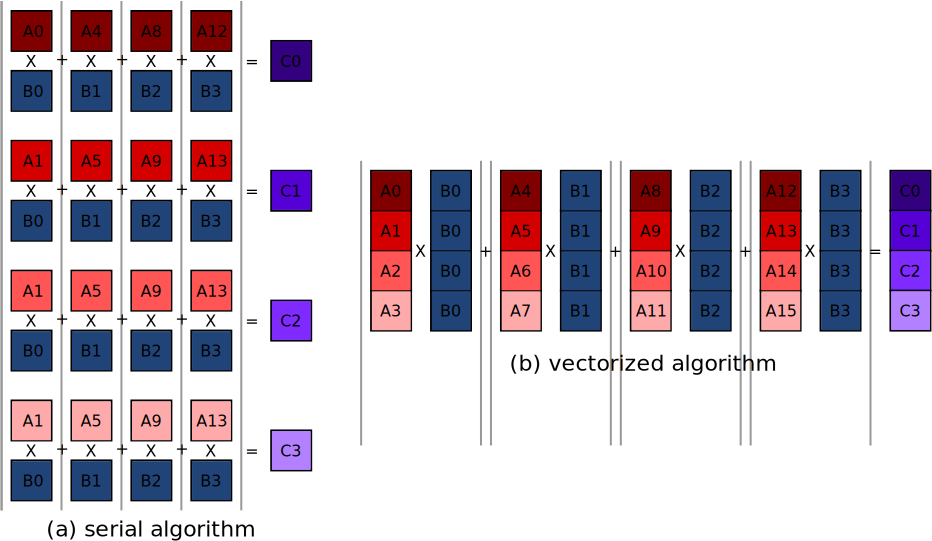
\includegraphics[width=\tw]{fig-opts-avx-vec.svg.pdf}

  \caption{\textbf{Overview of Vectorization Strategy --} For simplicity,
    4x4 matrices are shown with elements labeled in the column-major
    order. The computation required to generate the elements of a single
    column of the output matrix can be re-arranged to group multiple
    elements of the input matrix into a vector register. This effectively
    allows us to compute multiple elements of the output matrix in
    parallel (i.e., 4 doubles in parallel with 256b SIMD pipeline).}

  \label{fig-opts-avx-vec}

\end{figure}


As such, the goal of this optimization is to effectively utilize the SIMD
pipeline with AVX instructions. In order to do this, the first step is to
design a vectorization strategy for matrix
multiplication. Figure~\ref{fig-opts-avx-vec} outlines the
vectorization strategy used for this optimization.
\smallskip

If we consider the computations required to generate column {\tt{j}} of
matrix {\tt{C}}, we can see that all elements in column {\tt{k}} of matrix
{\tt{A}} need to be multiplied by $B_{kj}$. With this insight, we can
write the equation for computing a vector of elements in column {\tt{j}} of
matrix {\tt{C}} as follows:
\[
\{C_{0j},...,C_{Nj}\} = \sum_{k=0}^{N}\{A_{0k},...,A_{Nk}\}*B_{kj}
\]
\smallskip

By using vector registers to represent multiple elements of a given
column, we are able to vectorize computation across multiple elements
within a column of the output matrix.
\smallskip

The pseudo-assembly for computing one column of a block in the output
matrix is shown below:
\smallskip

\begin{verbatim}
    load.v  vr1, 0(c_addr) // vector load {C_0j,...,C_Nj} (partial product)
_loop:
    load.v  vr2, 0(a_addr) // vector load {A_0k,...,A_3k}
    load    r2,  0(b_addr) // load B_kj
    set.v   vr3, r2        // broadcast B_kj to vector register
    mul.v   vr4, vr2, vr3
    add.v   vr1, vr4, vr1
    addi    a_addr, inc    // pointer bump for A
    addi    b_addr, inc    // pointer bump for B
    br      _loop          // loop for N iterations
    store.v vr1, 0(c_addr) // vector store {C_0j,...,C_Nj}
\end{verbatim}
\smallskip

An alternative strategy would be to vectorize computation across
multiple elements within a \emph{row} of the output matrix. The challenge
with this approach is that since we would need to load multiple elements
within a row of matrices {\tt{B}} and {\tt{C}}, and since the matrices
are column-major in memory, we would have a stride of {\tt{N}} instead of
unit-stride as before. Not only would this be undesirable for cache
locality, it means we would be unable to utilize efficient vector loads,
which can only load elements that are consecutive in memory. However, in
order to evaluate the impact of regular vs. irregular memory accesses, we
have submitted both strategies for this assignment. These
implemementations are named {\tt{dgemm\_avx\_regular.c}} and
{\tt{dgemm\_avx\_irregular.c}}, respectively.
\smallskip

In addition to vectorizing matrix multiplication, AVX also has support
for fused floating-point multiply-adds (FMAs). Instead of having separate
instructions for the multiply and add in the pseudo-assembly above, FMAs
allow us to execute these operations as a single instruction. This
essentially doubles the throughput of floating-point operations in the
SIMD pipeline.
\smallskip

So far we have been assuming matrix dimensions that are evenly divisible
by 4, but there are some non-trivial complications that arise when this
is not the case. First, we cannot use standard vector memory operations
because they must always access \emph{256b-aligned addresses in
  memory}. We can always enforce this alignment during memory allocation
for the first column of a matrix, but if the dimensions are not evenly
divisible by the vector width, all subsequent columns are not guaranteed
to be aligned. To address this, we use \emph{unaligned} vector
memory operations which allow accesses to non-256b-aligned addresses, but are
not as efficient as the standard variants. Second, even with unaligned
vector memory operations, there is still the corner case when we want to
vector load the last elements in a column (i.e., the last 3 elements in a
column left to compute, but we vector load in groups of 4). We do not
want to modify any elements beyond the current column we are computing
lest we run the risk of storing junk data to the next column. To address
this, we use \emph{masked} vector memory operations that can specify which of
the 4 elements in memory should be accessed (i.e., only load the first 3
elements starting from the base address, instead of 4). However, masked
vector memory operations are even less efficient than the unaligned
variants.
\smallskip

A conservative approach would be to always calculate the mask and use the
masked vector memory operations. This would be slow, but would guarantee
correctness. A more aggressive approach would be to prioritize these
different types of vector memory operations in the order of highest efficiency
whenever possible:
\smallskip

\begin{itemize}
  \item Standard: for matrix dimensions divisible by 4
  \item Unaligned: for any matrix dimensions, when we are \emph{not}
    computing the last elements in a column
  \item Masked: for any matrix dimensions, when we are computing the last
    elements in a column
\end{itemize}
\medskip

% Results and analysis
\subsection{Results}
%=========================================================================
% fig-opts-avx-results.tex
%=========================================================================

\begin{figure}[b]

  \centering
  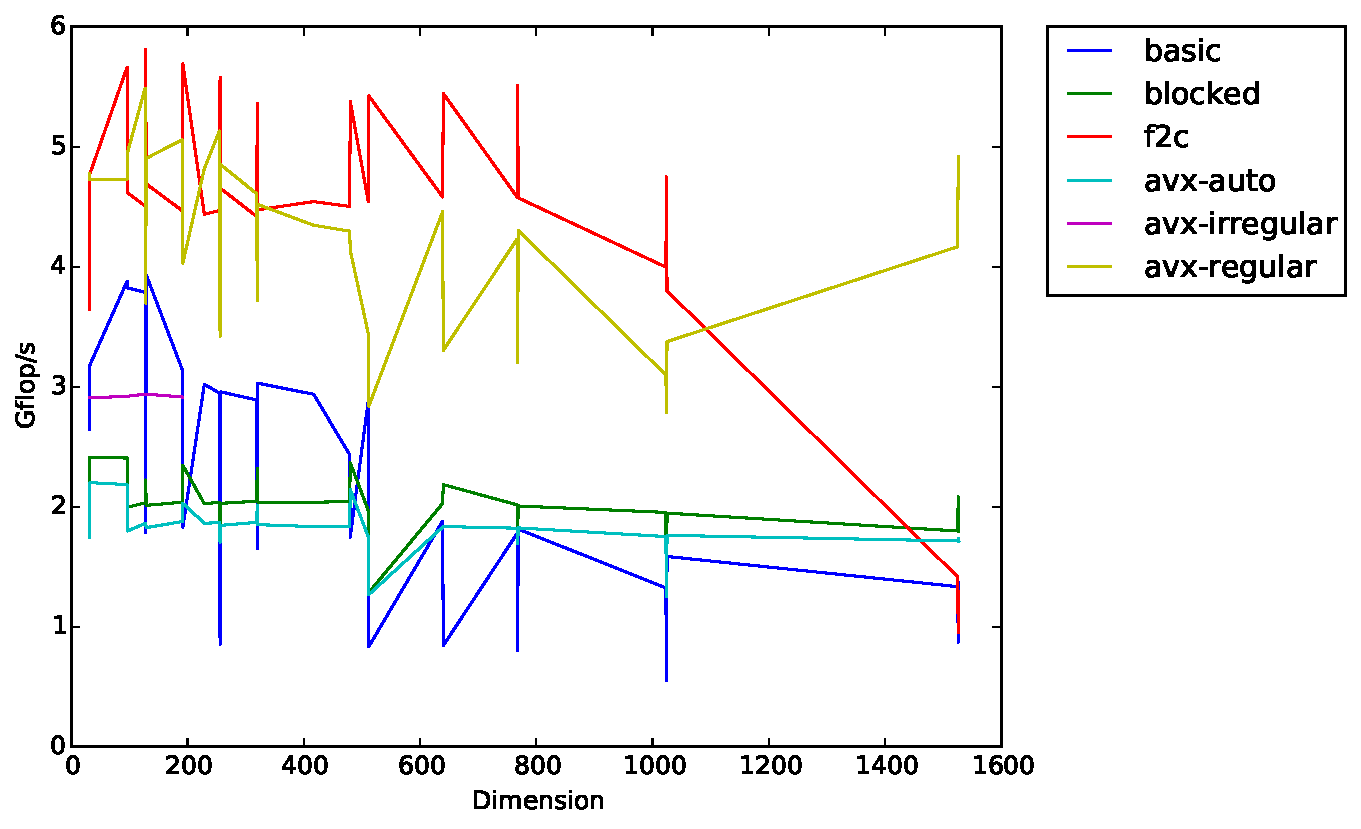
\includegraphics[width=0.7\tw]{fig-opts-avx-results.pdf}

  \caption{\textbf{Performance Comparison of AVX Optimizations --}
    Both AVX optimizations with the irregular and regular memory access
    patterns are shown. We intentionally omit the results for BLAS nad
    MKL implementations in order to focus on the behavior at the
    performance range of the optimization.}

  \label{fig-opts-avx-results}

\end{figure}


We evaluate both the regular and irregular memory access variants of the
vectorizing optimization with FMAs and support for any matrix dimension
using masked vector memory operations. In order to quantify the benefit
of manual-vectorization over auto-vectorization, we show the performance
of the provided blocked implementation using the {\tt{-xAVX}} compiler
flag. The results of using a combination of manual- and
auto-vectorization were also collected. All results are shown in
Figure~\ref{fig-opts-avx-results}.
\smallskip

The regular variant showed the better speedup of ~3x over the naive
blocked implementation. In contrast, the irregular variant had a slowdown
of roughly ~2x over the same baseline, highlighting the importance of
prioritizing desirable cache access patterns as well as efficient vector
memory operations. In addition, we can see that auto-vectorization is
significantly worse than manual-vectorization, but combining both
techniques outperforms either. This makes sense, since there are still
opportunities for vectorization that are not exploited with
manual-vectorization that is easier for the compiler to optimize.
\smallskip


Since we are using doubles (64b) for data elements and the SIMD pipeline
is 256b wide, we know we can fit 4 elements per vector register. In the
ideal case where the matrix dimension is evenly divisible by 4, we are
parallelizing computation over 4 elements of the output matrix. Coupled
with the use of FMAs which double the throughput of floating-point
operations in the SIMD pipeline, the ideal speedup should be ~8x. There
are several factors that prevent us from reaching this limit. For one,
the ideal speedup does not take into account the cache misses and
thrashing that occurs in practice. There is also the overhead from
copying scalar registers to vector registers, as well as the mask
calculation for masked vector memory operations. The overhead from
conditional blocks for prioritizing different types of vector memory
operations is non-trivial as well.

%\clearpage
